% !Mode:: "TeX:ACP:Hard"
\documentclass[14pt,hyperref={CJKbookmarks=true}]{beamer}

%\usepackage[space,noindent]{ctex}
\usepackage{mathrsfs}
\usepackage{amsfonts,amssymb}
\usepackage{amsmath}
\usepackage{graphicx}
\usepackage{subcaption}
\usepackage{lmodern}
\usepackage[labelformat=empty,font=scriptsize,skip=0pt,justification=justified,singlelinecheck=false]{caption}
\usepackage{amsthm}
\usepackage{color}
\usepackage{multimedia}

\theoremstyle{plain}
\newtheorem{thm}{Theorem}[section]
\newtheorem{lem}[thm]{Lemma}
\newtheorem{prop}[thm]{Proposition}
\newtheorem*{cor}{Corollary}

\theoremstyle{definition}
\newtheorem{defn}{Definition}[section]
\newtheorem{conj}{Conjecture}[section]
\newtheorem{exmp}{Example}[section]

\theoremstyle{remark}
\newtheorem*{rem}{Remark}

%\captionsetup{font={scriptsize}}
\captionsetup[figure]{name=Fig., labelsep=space}
%remove the icon
\setbeamertemplate{bibliography item}{}
%remove line breaks
\setbeamertemplate{bibliography entry title}{}
\setbeamertemplate{bibliography entry location}{}
\setbeamertemplate{bibliography entry note}{}
%\usetheme{AnnArbor}
\usetheme{CambridgeUS}
%\usetheme{Berlin}
%\usetheme{Dresden}
%\usecolortheme{beaver}
%\setbeamercolor{itemize item}{fg=black!80!black}

\setbeamercolor{normal text}{bg=black!10}
\setbeamerfont{caption}{size=\tiny}
\graphicspath{{./image/}}

\begin{document}

%\section{Title}
\title[IACAS]{Extended Kalman Filter and its Application}
%\subtitle[副题简称]{论文副题}
\author{Tian Chen}
\institute[]{Institute of Automation Chinese Academy of Sciences\\University of Chinese Academy of Sciences}
\date[]{2017.04.13}
\begin{frame}
\titlepage
\end{frame}


%% Outline page
\begin{frame}
\frametitle{Quick Overview}
\large\tableofcontents
\end{frame}

%%
\section{Introduction}
\begin{frame}
\frametitle{Introduction}
\small
\begin{block}{Bayes}
\begin{equation}
  P(x|y) =\frac{P(xy)}{P(y)}
\end{equation}

\end{block}


\end{frame}
\begin{frame}

%\begin{figure}[h!]
%\centering
%\movie[label=show3,width=1.0\textwidth,poster
%       ,autostart,showcontrols,loop]
%  {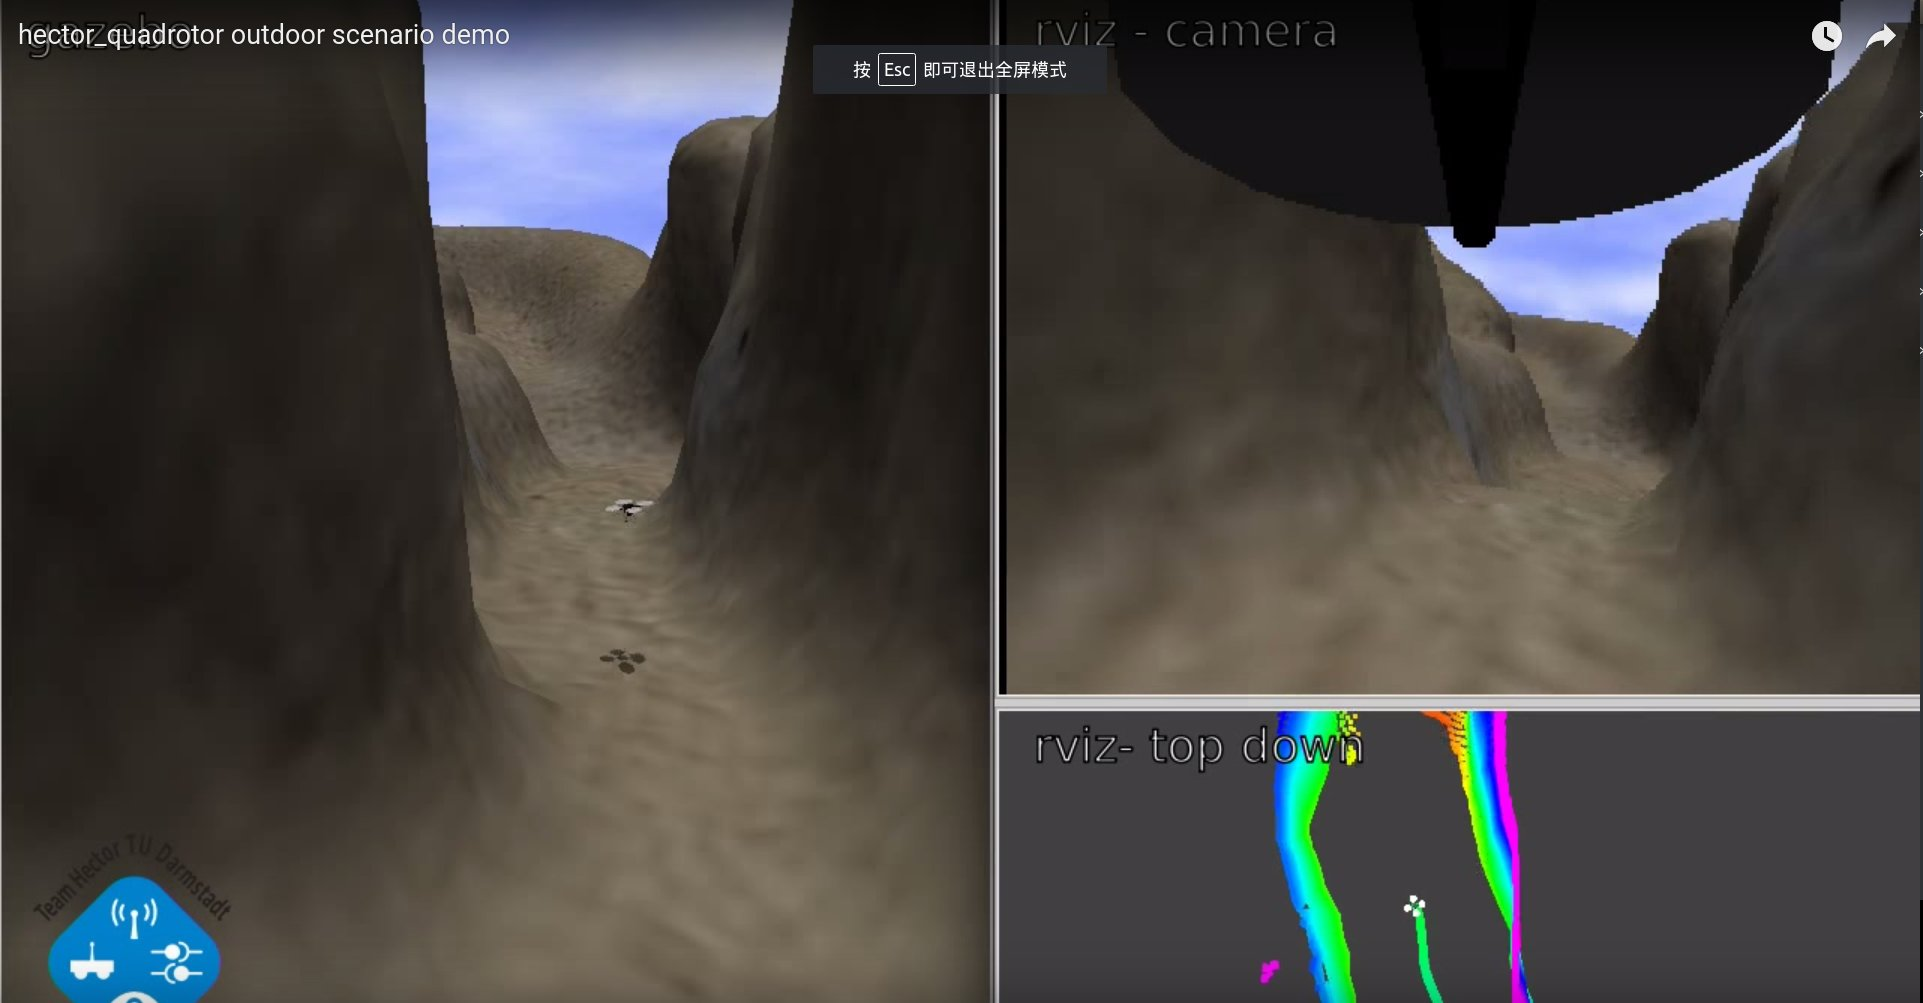
\includegraphics[width=1.0\textwidth]{squashscreen.jpg}}{landing.avi}
%  \caption{caption}
% \end{figure}
\end{frame}


\section{Method}

\begin{frame}
\small
\frametitle{Method}{EKF}
\begin{block}{Problems}
\begin{itemize}
\item xx
\end{itemize}
\end{block}
\end{frame}


\section{Experiment}
\begin{frame}
\frametitle{Experiment}
\begin{block}{The slam System}
\begin{enumerate}
\item xx
\end{enumerate}
\end{block}
\end{frame}


\section{Conclusion}
\begin{frame}{Conclusion}
\small
\begin{enumerate}
\item  x
\end{enumerate}
\end{frame}
%\section{Thanks}
\begin{frame}
%\frametitle{Thank you}
\Huge
\begin{center}
Thank you
\end{center}


%\begin{block}{Collaborators}
%De Xu, Zhengtao Zhang and Dapeng Zhang
%\end{block}
%\begin{block}{Foundation}
% National Nature Science Foundation under Grant 61473293, 61227804 and 61303177
%\end{block}
%\begin{block}{For more information about the research itself:}
%De Xu, Zhengtao Zhang and Dapeng Zhang
%Institute of Automation, Chinese Academy of Sciences, Beijing 100190
%E-mail: dingwendong2013@ia.ac.cn
%\end{block}
\end{frame}
\end{document}
